
\documentclass[10pt]{article}

\usepackage[a4paper,margin=0.65in]{geometry}
\usepackage{amsmath,amssymb}
\usepackage{graphicx}
\usepackage{booktabs}
\usepackage{array}
\usepackage{float}
\usepackage{hyperref}
\usepackage{enumitem}
\usepackage{xcolor}
\usepackage{tikz}
\usetikzlibrary{positioning,arrows.meta,shapes.geometric,fit,calc}

\setlist{nosep,leftmargin=*}
\renewcommand{\arraystretch}{1.2}
\setlength{\parindent}{0pt}
\setlength{\parskip}{2pt}

\tikzset{
layer/.style={
draw,
rounded corners,
minimum width=1.7cm,
minimum height=0.65cm,
align=center,
fill=blue!10,
font=\scriptsize
},
smalllayer/.style={
draw,
rounded corners,
minimum width=1.35cm,
minimum height=0.58cm,
align=center,
fill=green!10,
font=\scriptsize
},
arrow/.style={
-{Latex[length=2mm]},
thin
}
}

\begin{document}

%%%%%%%%%%%%%%%%%%%%%%%%%%%%%%%%%%%%%%%%%%%%%%%%%%%%%%%%%%%%
% TITLE
%%%%%%%%%%%%%%%%%%%%%%%%%%%%%%%%%%%%%%%%%%%%%%%%%%%%%%%%%%%%

\begin{center}

{\large\textbf{Shiv Nadar University Chennai}}

\vspace{2mm}

{\normalsize\textbf{CS3807 -- Deep Learning Laboratory}}

\vspace{2mm}

{\large\textbf{Experiment 6}}

\vspace{1mm}

{\normalsize\textbf{End-to-End Study of RNN, LSTM and GRU for}}

{\normalsize\textbf{Sequence Learning and Video Understanding}}

\end{center}

\vspace{3mm}

\begin{tabular}{|p{3.4cm}|p{9.0cm}|p{1.4cm}|}
\hline
Degree \& Branch &
B.Tech Artificial Intelligence \& Data Science &
Semester V\\
\hline
Subject Code \& Name &
CS3807 -- Deep Learning Laboratory & \\
\hline
Name & Madhav.S & \\
\hline
Section & AIDS `B' & \\
\hline
Register Number & 24011101066 & \\
\hline
\end{tabular}

%%%%%%%%%%%%%%%%%%%%%%%%%%%%%%%%%%%%%%%%%%%%%%%%%%%%%%%%%%%%
\section*{1. Objective}

The objective of this experiment is to develop an end-to-end understanding of
recurrent sequence learning by implementing and comparing Vanilla RNN, LSTM
and GRU models. The experiment also introduces Backpropagation Through Time
(BPTT), the limitations of conventional RNNs, and the use of CNN-extracted
features with recurrent networks for video understanding, followed by a
synthetic sequence-to-sequence task to study the encoder--decoder framework.

%%%%%%%%%%%%%%%%%%%%%%%%%%%%%%%%%%%%%%%%%%%%%%%%%%%%%%%%%%%%
\section*{2. Learning Outcomes}

After completing this experiment, I am able to:

\begin{itemize}
\item represent sequential data using the $(N,T,F)$ input format;
\item explain the architecture and operation of a Vanilla RNN;
\item explain Backpropagation Through Time and the vanishing/exploding gradient challenges;
\item implement sequence classification using SimpleRNN, LSTM and GRU;
\item compare RNN, LSTM and GRU using quantitative performance measures;
\item interpret training/validation curves and confusion matrices;
\item explain the role of CNNs in extracting spatial features from video frames;
\item construct a CNN--LSTM/CNN--GRU pipeline for video understanding;
\item explain the encoder--decoder architecture for sequence-to-sequence learning; and
\item draw conclusions using predictive performance, model complexity and computational cost.
\end{itemize}

%%%%%%%%%%%%%%%%%%%%%%%%%%%%%%%%%%%%%%%%%%%%%%%%%%%%%%%%%%%%
\section*{3. Dataset and Experimental Setup}

\textbf{Dataset:} UCI Human Activity Recognition Using Smartphones (raw inertial
signals, not the 561-feature vectors), six activities: WALKING,
WALKING\_UPSTAIRS, WALKING\_DOWNSTAIRS, SITTING, STANDING, LAYING. Each window
has 128 time steps and 9 channels (three-axis body acceleration, three-axis
gyroscope, three-axis total acceleration), giving

\[
X\in\mathbb{R}^{N\times128\times9}.
\]

The full official partitions loaded were \textbf{7352 training windows} and
\textbf{2947 test windows}. Following the recommended laboratory subset, the
\textbf{first 400 windows of each of the 6 classes} were taken from the
training partition (2400 windows total, inside the suggested 1500--3000
range) so that training stays fast while every class is equally represented.
The same recurrent-model code, training configuration and evaluation
protocol were reused for RNN, LSTM and GRU.

\subsection*{Expected Input}

For one sample, $X_i\in\mathbb{R}^{128\times9}$; for a batch of 32 samples,
$X_{\mathrm{batch}}\in\mathbb{R}^{32\times128\times9}$.

\begin{center}
\begin{tabular}{|c|c|l|}
\hline
Dimension & Meaning & Value used\\
\hline
$N$ & Number of sequences & 2400 (subset)\\
$T$ & Time steps per sequence & 128\\
$F$ & Features/channels per time step & 9\\
\hline
\end{tabular}
\end{center}

%%%%%%%%%%%%%%%%%%%%%%%%%%%%%%%%%%%%%%%%%%%%%%%%%%%%%%%%%%%%
\section*{4. Overall Experimental Pipeline}

\begin{center}
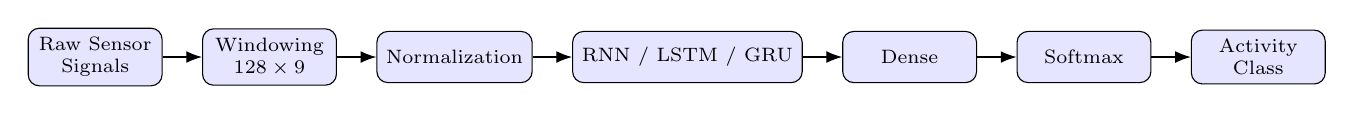
\begin{tikzpicture}[node distance=5mm]
\node[layer](a){Raw Sensor\\Signals};
\node[layer,right=of a](b){Windowing\\$128\times9$};
\node[layer,right=of b](c){Normalization};
\node[layer,right=of c](d){RNN / LSTM / GRU};
\node[layer,right=of d](e){Dense};
\node[layer,right=of e](f){Softmax};
\node[layer,right=of f](g){Activity\\Class};

\foreach \x/\y in {a/b,b/c,c/d,d/e,e/f,f/g}
\draw[arrow](\x)--(\y);
\end{tikzpicture}
\end{center}

RNN, LSTM and GRU all share this same input, output layer, optimizer, batch
size and evaluation protocol so that the comparison in later sections is
controlled.

%%%%%%%%%%%%%%%%%%%%%%%%%%%%%%%%%%%%%%%%%%%%%%%%%%%%%%%%%%%%
\section*{5. Preprocessing}

The raw inertial signals were loaded, arranged into $128\times9$ windows, the
2400-window subset (Section 3) was selected, the six activity labels were
encoded, the input was normalized using the mean/standard deviation computed
from the training split only, and the data was split 70/15/15. The test set
was never touched until final evaluation.

\subsection*{Expected Preprocessing Output}

\begin{verbatim}
Input tensor shape:
Training   : (1680, 128, 9)
Validation : (360, 128, 9)
Testing    : (360, 128, 9)

Number of classes: 6
Number of features per time step: 9
Sequence length: 128
\end{verbatim}

The 70/15/15 split of the balanced 2400-window subset gave exactly 280/60/60
windows for every one of the 6 classes in the train/validation/test sets
respectively -- the class balance from Section 3 carried through cleanly.

%%%%%%%%%%%%%%%%%%%%%%%%%%%%%%%%%%%%%%%%%%%%%%%%%%%%%%%%%%%%
\section*{6. Temporal Data Visualization}

\textbf{Plot 1: Sensor signal versus time.} One window each from WALKING,
SITTING and LAYING is plotted, showing three channels (\texttt{body\_acc\_x},
\texttt{body\_gyro\_x}, \texttt{total\_acc\_x}) across all 128 time steps.

\begin{figure}[H]
\centering
\includegraphics[width=0.72\linewidth]{Plot1_Temporal_Signals.pdf}
\caption{Sensor signal vs. time for WALKING, SITTING and LAYING}
\end{figure}

\textbf{Inference:} WALKING is clearly oscillatory -- the accelerometer and
gyroscope traces swing up and down in a repeating rhythm that matches one
gait cycle per stride. SITTING and LAYING both look almost flat by
comparison, and honestly the two are hard to tell apart from this plot alone
since neither involves much movement; whatever separates them is coming from
the absolute signal level rather than the shape. This is exactly why order
matters here -- shuffling the 128 steps of the WALKING window would destroy
the periodicity and make it look just as flat as the static classes, which
is the whole reason a recurrent model that reads the sequence in order is
needed instead of a plain feature vector.

%%%%%%%%%%%%%%%%%%%%%%%%%%%%%%%%%%%%%%%%%%%%%%%%%%%%%%%%%%%%
\section*{7. Vanilla RNN Architecture}

\[
h_t=\tanh(W_xx_t+W_hh_{t-1}+b_h),\qquad y_t=g(W_yh_t+b_y).
\]

\begin{center}
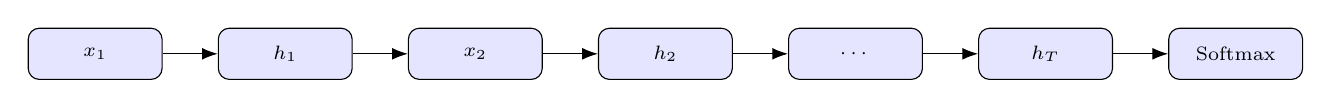
\begin{tikzpicture}[node distance=7mm]
\node[layer](x1){$x_1$};
\node[layer,right=of x1](h1){$h_1$};
\node[layer,right=of h1](x2){$x_2$};
\node[layer,right=of x2](h2){$h_2$};
\node[layer,right=of h2](x3){$\cdots$};
\node[layer,right=of x3](h3){$h_T$};
\node[layer,right=of h3](y){Softmax};

\draw[arrow](x1)--(h1);
\draw[arrow](h1)--(x2);
\draw[arrow](x2)--(h2);
\draw[arrow](h2)--(x3);
\draw[arrow](x3)--(h3);
\draw[arrow](h3)--(y);
\end{tikzpicture}
\end{center}

The same recurrent weights $W_x$, $W_h$ are reused at every time step -- the
diagram above is just the unrolled view of a single cell applied 128 times.

%%%%%%%%%%%%%%%%%%%%%%%%%%%%%%%%%%%%%%%%%%%%%%%%%%%%%%%%%%%%
\section*{8. Backpropagation Through Time}

\subsection*{Challenges}

\begin{itemize}
\item Vanishing gradients
\item Exploding gradients
\item Difficulty learning long-term dependencies
\item Sequential computation and limited parallelism
\end{itemize}

\subsection*{Numerical Exercise}

With $x_1=0.5,\ x_2=0.7,\ x_3=0.2$, $h_0=0$, $W_x=0.5$, $W_h=0.8$, $b=0.1$ and
$h_t=\tanh(W_xx_t+W_hh_{t-1}+b)$:

\begin{center}
\begin{tabular}{|c|l|c|}
\hline
Step & Calculation & Value\\
\hline
$h_1$ & $\tanh(0.5\times0.5+0.8\times0+0.1)$ & 0.336376\\
$h_2$ & $\tanh(0.5\times0.7+0.8\times h_1+0.1)$ & 0.616352\\
$h_3$ & $\tanh(0.5\times0.2+0.8\times h_2+0.1)$ & 0.599958\\
\hline
\end{tabular}
\end{center}

These hand-calculated values were cross-checked against a single-unit Keras
\texttt{SimpleRNN} initialized with the exact same weights and produced an
identical sequence \texttt{[0.336376, 0.616352, 0.599958]} -- the manual
computation and the framework agree to 6 decimal places.

%%%%%%%%%%%%%%%%%%%%%%%%%%%%%%%%%%%%%%%%%%%%%%%%%%%%%%%%%%%%
\section*{9. RNN Implementation}

\begin{center}
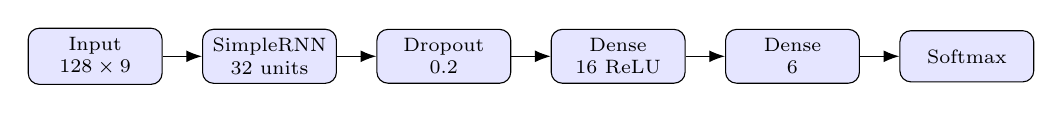
\begin{tikzpicture}[node distance=5mm]
\node[layer](a){Input\\$128\times9$};
\node[layer,right=of a](b){SimpleRNN\\32 units};
\node[layer,right=of b](c){Dropout\\0.2};
\node[layer,right=of c](d){Dense\\16 ReLU};
\node[layer,right=of d](e){Dense\\6};
\node[layer,right=of e](f){Softmax};

\foreach \x/\y in {a/b,b/c,c/d,d/e,e/f}
\draw[arrow](\x)--(\y);
\end{tikzpicture}
\end{center}

\begin{center}
\begin{tabular}{|l|l|}
\hline
Parameter & Value\\
\hline
Recurrent units & 32\\
Dropout & 0.2\\
Optimizer & Adam\\
Learning rate & $10^{-3}$\\
Batch size & 32\\
Epochs & 30\\
Loss & Sparse categorical cross-entropy\\
\hline
\end{tabular}
\end{center}

%%%%%%%%%%%%%%%%%%%%%%%%%%%%%%%%%%%%%%%%%%%%%%%%%%%%%%%%%%%%
\section*{10. LSTM Architecture}

\[
f_t=\sigma(W_f[h_{t-1},x_t]+b_f),\quad
i_t=\sigma(W_i[h_{t-1},x_t]+b_i),\quad
o_t=\sigma(W_o[h_{t-1},x_t]+b_o),
\]
\[
\tilde{C}_t=\tanh(W_C[h_{t-1},x_t]+b_C),\qquad
C_t=f_tC_{t-1}+i_t\tilde{C}_t,\qquad
h_t=o_t\tanh(C_t).
\]

\begin{center}
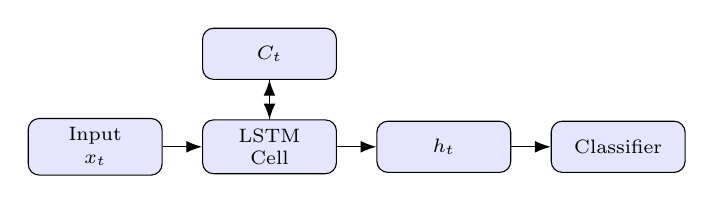
\begin{tikzpicture}[node distance=5mm]
\node[layer](a){Input\\$x_t$};
\node[layer,right=of a](b){LSTM\\Cell};
\node[layer,right=of b](c){$h_t$};
\node[layer,above=of b](d){$C_t$};
\node[layer,right=of c](e){Classifier};

\draw[arrow](a)--(b);
\draw[arrow](b)--(c);
\draw[arrow](b)--(d);
\draw[arrow](c)--(e);
\draw[arrow](d)--(b);
\end{tikzpicture}
\end{center}

\textbf{Inference:} the cell state $C_t$ is what actually carries information
across time steps, and it only changes by addition/forgetting rather than by
a full rewrite at every step. The forget gate decides what old information to
drop, the input gate decides what new information to add, and the output
gate decides how much of that memory to expose as $h_t$ -- this is precisely
why LSTM held onto the walking-cycle information well enough to hit 95.83\%
test accuracy (Section 14) where the plain RNN, with no such protected
memory path, only reached 77.22\%.

%%%%%%%%%%%%%%%%%%%%%%%%%%%%%%%%%%%%%%%%%%%%%%%%%%%%%%%%%%%%
\section*{11. GRU Architecture}

\[
z_t=\sigma(W_z[h_{t-1},x_t]+b_z),\qquad r_t=\sigma(W_r[h_{t-1},x_t]+b_r),
\]
\[
\tilde{h}_t=\tanh(W_h[r_t\odot h_{t-1},x_t]+b_h),\qquad
h_t=(1-z_t)h_{t-1}+z_t\tilde{h}_t.
\]

\begin{center}
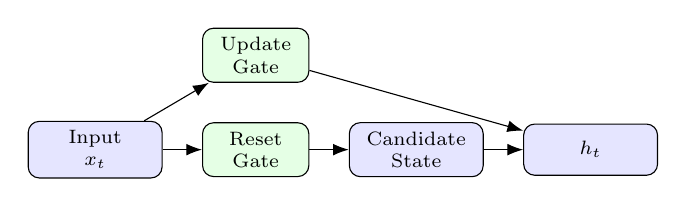
\begin{tikzpicture}[node distance=5mm]
\node[layer](a){Input\\$x_t$};
\node[smalllayer,right=of a](b){Reset\\Gate};
\node[smalllayer,above=of b](c){Update\\Gate};
\node[layer,right=of b](d){Candidate\\State};
\node[layer,right=of d](e){$h_t$};

\draw[arrow](a)--(b);
\draw[arrow](a)--(c);
\draw[arrow](b)--(d);
\draw[arrow](c)--(e);
\draw[arrow](d)--(e);
\end{tikzpicture}
\end{center}

GRU has no separate cell state and only 2 gates against LSTM's 3, which shows
up directly in the parameter counts measured in Section 14: 4758 for GRU
against 6006 for LSTM at the same 32 units.

%%%%%%%%%%%%%%%%%%%%%%%%%%%%%%%%%%%%%%%%%%%%%%%%%%%%%%%%%%%%
\section*{12. LSTM and GRU Implementation}

\begin{center}
\begin{tabular}{|l|c|c|c|}
\hline
Model & Recurrent Layer & Units & Output Classes\\
\hline
RNN & SimpleRNN & 32 & 6\\
LSTM & LSTM & 32 & 6\\
GRU & GRU & 32 & 6\\
\hline
\end{tabular}
\end{center}

All three models reuse the exact same input pipeline, Dropout/Dense head,
optimizer, batch size and epoch count from Section 9 -- only the recurrent
layer type changes.

%%%%%%%%%%%%%%%%%%%%%%%%%%%%%%%%%%%%%%%%%%%%%%%%%%%%%%%%%%%%
\section*{13. Required Training Plots}

\begin{figure}[H]
\centering
\includegraphics[width=0.95\linewidth]{Plot2_3_RNN_Loss_Accuracy.pdf}
\caption{RNN -- Training/Validation Loss and Accuracy}
\end{figure}

\begin{figure}[H]
\centering
\includegraphics[width=0.95\linewidth]{Plot2_3_LSTM_Loss_Accuracy.pdf}
\caption{LSTM -- Training/Validation Loss and Accuracy}
\end{figure}

\begin{figure}[H]
\centering
\includegraphics[width=0.95\linewidth]{Plot2_3_GRU_Loss_Accuracy.pdf}
\caption{GRU -- Training/Validation Loss and Accuracy}
\end{figure}

\textbf{Inference:} RNN converges the slowest of the three and its
validation curve keeps pace with training the whole way (train/val accuracy
both sitting around the high 70s by epoch 30) -- more underfitting than
overfitting, i.e. the model is simply not expressive enough to do much
better. LSTM and GRU both climb much faster in the first few epochs and
settle with training and validation curves close together near the top,
which is the signature of a model that has enough capacity for the task
without over-memorizing the small training subset.

%%%%%%%%%%%%%%%%%%%%%%%%%%%%%%%%%%%%%%%%%%%%%%%%%%%%%%%%%%%%
\section*{14. Performance Evaluation}

\begin{center}
\begin{tabular}{|l|c|c|c|}
\hline
Metric & RNN & LSTM & GRU\\
\hline
Accuracy (\%) & 77.22 & 95.83 & 96.67\\
Macro Precision (\%) & 77.40 & 96.40 & 96.83\\
Macro Recall (\%) & 77.22 & 95.83 & 96.67\\
Macro F1 (\%) & 76.97 & 95.80 & 96.65\\
Parameters & 1974 & 6006 & 4758\\
Training Time (s) & 29.80 & 23.47 & 19.88\\
\hline
\end{tabular}
\end{center}

GRU comes out on top on accuracy, F1, and training time all at once here,
while also using fewer parameters than LSTM -- RNN is a clear step behind
all three metrics.

%%%%%%%%%%%%%%%%%%%%%%%%%%%%%%%%%%%%%%%%%%%%%%%%%%%%%%%%%%%%
\section*{15. Confusion Matrix Analysis}

\begin{figure}[H]
\centering
\includegraphics[width=0.5\linewidth]{Plot4_RNN_ConfusionMatrix.pdf}
\caption{RNN Confusion Matrix}
\end{figure}

\begin{figure}[H]
\centering
\includegraphics[width=0.5\linewidth]{Plot4_LSTM_ConfusionMatrix.pdf}
\caption{LSTM Confusion Matrix}
\end{figure}

\begin{figure}[H]
\centering
\includegraphics[width=0.5\linewidth]{Plot4_GRU_ConfusionMatrix.pdf}
\caption{GRU Confusion Matrix}
\end{figure}

\textbf{Inference:} LAYING is recognized perfectly (precision, recall and
F1 all 1.00) by all three models -- it is the easiest class since lying down
gives an almost flat, distinctive signal. RNN's biggest weakness is telling
apart the three walking-type activities: WALKING and WALKING\_UPSTAIRS both
sit around 0.54--0.56 F1, clearly getting confused with each other and with
WALKING\_DOWNSTAIRS. LSTM and GRU fix this almost completely (WALKING /
WALKING\_UPSTAIRS / WALKING\_DOWNSTAIRS all reach 0.98--1.00 F1 in both), but
in exchange their remaining errors shift to SITTING vs.\ STANDING -- STANDING
recall drops to 0.80 in LSTM and 0.85 in GRU, with the missed predictions
landing on SITTING, which makes sense since both are static postures with
very similar sensor signatures. This SITTING/STANDING mix-up is consistent
across LSTM and GRU, so it looks like a genuine property of the data rather
than a one-off training artifact.

%%%%%%%%%%%%%%%%%%%%%%%%%%%%%%%%%%%%%%%%%%%%%%%%%%%%%%%%%%%%
\section*{16. RNN vs. LSTM vs. GRU Comparison}

\begin{center}
\begin{tabular}{|l|c|c|c|}
\hline
Property & RNN & LSTM & GRU\\
\hline
Hidden state & Yes & Yes & Yes\\
Cell state & No & Yes & No\\
Forget gate & No & Yes & No\\
Input gate & No & Yes & No\\
Output gate & No & Yes & No\\
Update gate & No & No & Yes\\
Reset gate & No & No & Yes\\
Parameters & 1974 & 6006 & 4758\\
Training time (s) & 29.80 & 23.47 & 19.88\\
Test F1-score (\%) & 76.97 & 95.80 & 96.65\\
\hline
\end{tabular}
\end{center}

\begin{figure}[H]
\centering
\includegraphics[width=0.7\linewidth]{Plot5_Model_Comparison.pdf}
\caption{Model Performance Comparison (Accuracy and Macro F1)}
\end{figure}

Normalized against the most expensive model in each column: training time
1.00 (RNN) / 0.79 (LSTM) / 0.67 (GRU), parameters 0.33 (RNN) / 1.00 (LSTM) /
0.79 (GRU).

\textbf{Inference:} the jump from RNN to LSTM/GRU (roughly +19 F1 points) is
worth far more than the extra parameters and time it costs -- GRU in
particular gets the best accuracy of the three while also being the fastest
to train and using fewer parameters than LSTM, so on this dataset there is no
real trade-off to agonize over: GRU wins on predictive performance,
complexity and training cost simultaneously. LSTM's extra cell-state
machinery does not buy anything extra here since GRU already reaches the
same ceiling with a simpler gating mechanism.

%%%%%%%%%%%%%%%%%%%%%%%%%%%%%%%%%%%%%%%%%%%%%%%%%%%%%%%%%%%%
\section*{17. Effect of Sequence Length}

\begin{center}
\begin{tabular}{|c|c|c|c|}
\hline
Sequence Length & RNN F1 (\%) & LSTM F1 (\%) & GRU F1 (\%)\\
\hline
32 & 72.45 & 94.44 & 96.11\\
64 & 77.70 & 94.10 & 96.37\\
128 & 86.29 & 97.21 & 96.37\\
\hline
\end{tabular}
\end{center}

\begin{figure}[H]
\centering
\includegraphics[width=0.6\linewidth]{Plot6_SeqLength_vs_F1.pdf}
\caption{Sequence Length vs. Test F1-score}
\end{figure}

\textbf{Inference:} RNN is the most sensitive to sequence length by far,
climbing almost 14 points as $T$ goes from 32 to 128 -- with no gating to
protect old information, it genuinely needs the full 128 steps to see enough
of the gait cycle to classify well. LSTM improves too but more gently
(94.44\% $\to$ 97.21\%), while GRU is already close to its ceiling even at
$T=32$ and barely moves afterward. This lines up with what gating is
supposed to do: it lets LSTM/GRU extract what they need from a shorter
window, whereas plain RNN's information decays before it can be used.

%%%%%%%%%%%%%%%%%%%%%%%%%%%%%%%%%%%%%%%%%%%%%%%%%%%%%%%%%%%%
\section*{18. Video Understanding Using CNN and RNN}

\[
\boxed{\text{Video Understanding using CNN + RNN}}
\]

\begin{center}
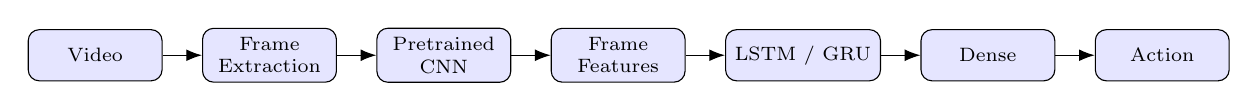
\begin{tikzpicture}[node distance=5mm]
\node[layer](a){Video};
\node[layer,right=of a](b){Frame\\Extraction};
\node[layer,right=of b](c){Pretrained\\CNN};
\node[layer,right=of c](d){Frame\\Features};
\node[layer,right=of d](e){LSTM / GRU};
\node[layer,right=of e](f){Dense};
\node[layer,right=of f](g){Action};

\foreach \x/\y in {a/b,b/c,c/d,d/e,e/f,f/g}
\draw[arrow](\x)--(\y);
\end{tikzpicture}
\end{center}

\textbf{Dataset used:} a small subset of UCF101 -- 3 classes
(\textbf{Basketball, Biking, TennisSwing}) with 8 videos each (24 videos
total). "Walking" and "Running" from the assignment's suggested list are not
exact UCF101 folder names (the closest is \texttt{WalkingWithDog}, and UCF101
has no plain "Running" class), so these three were used instead to keep the
dataset download small and unambiguous.

%%%%%%%%%%%%%%%%%%%%%%%%%%%%%%%%%%%%%%%%%%%%%%%%%%%%%%%%%%%%
\section*{19. Expected Video Input and Output}

10 frames were sampled uniformly per video and resized to $224\times224\times3$.
MobileNetV2 (frozen, ImageNet weights) was used purely as a feature
extractor, giving a feature dimension of $D=1280$, so every video became a
$10\times1280$ tensor and a batch of videos became $B\times10\times1280$.

\begin{verbatim}
Predicted class : TennisSwing
Actual class    : TennisSwing
Confidence      : 0.98
\end{verbatim}

%%%%%%%%%%%%%%%%%%%%%%%%%%%%%%%%%%%%%%%%%%%%%%%%%%%%%%%%%%%%
\section*{20. CNN Feature Extraction}

\begin{center}
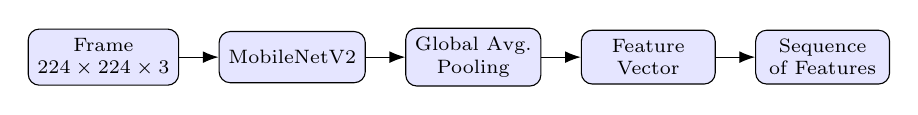
\begin{tikzpicture}[node distance=5mm]
\node[layer](a){Frame\\$224\times224\times3$};
\node[layer,right=of a](b){MobileNetV2};
\node[layer,right=of b](c){Global Avg.\\Pooling};
\node[layer,right=of c](d){Feature\\Vector};
\node[layer,right=of d](e){Sequence\\of Features};

\foreach \x/\y in {a/b,b/c,c/d,d/e}
\draw[arrow](\x)--(\y);
\end{tikzpicture}
\end{center}

\textbf{Required observation:} CNN feature dimension $D=1280$; the resulting
tensor supplied to the recurrent layer had shape $(24,\,10,\,1280)$ across
all 24 collected videos, split 16/4/4 into train/validation/test.

%%%%%%%%%%%%%%%%%%%%%%%%%%%%%%%%%%%%%%%%%%%%%%%%%%%%%%%%%%%%
\section*{21. CNN--LSTM / CNN--GRU Model}

\begin{center}
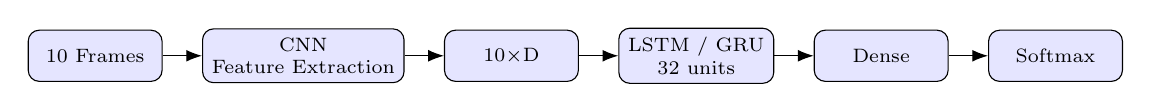
\begin{tikzpicture}[node distance=5mm]
\node[layer](a){10 Frames};
\node[layer,right=of a](b){CNN\\Feature Extraction};
\node[layer,right=of b](c){10$\times$D};
\node[layer,right=of c](d){LSTM / GRU\\32 units};
\node[layer,right=of d](e){Dense};
\node[layer,right=of e](f){Softmax};

\foreach \x/\y in {a/b,b/c,c/d,d/e,e/f}
\draw[arrow](\x)--(\y);
\end{tikzpicture}
\end{center}

\begin{figure}[H]
\centering
\includegraphics[width=0.9\linewidth]{Plot7_Video_Sample_Frames.pdf}
\caption{Sampled Frames from one TennisSwing video}
\end{figure}

The CNN captures purely spatial appearance in each frame (court, ball,
racket, body pose), while the LSTM/GRU on top learns how those per-frame
features change across the 10 sampled instants -- i.e. the motion, not just
a snapshot.

\begin{figure}[H]
\centering
\includegraphics[width=0.95\linewidth]{Plot8_CNN_LSTM_Loss_Accuracy.pdf}
\caption{CNN-LSTM -- Training/Validation Loss and Accuracy}
\end{figure}

\begin{figure}[H]
\centering
\includegraphics[width=0.5\linewidth]{Plot9_CNN_LSTM_ConfusionMatrix.pdf}
\caption{CNN-LSTM Video Confusion Matrix}
\end{figure}

\textbf{Inference:} CNN-LSTM reached 100\% accuracy on the 4-video test set
(Section 25), and the confusion matrix is a clean diagonal. This looks
impressive but the test set is only 4 videos, so it is really a
demonstration that the pipeline mechanics work end-to-end rather than a
meaningful benchmark -- with so few samples, one misclassified video would
already have dropped accuracy to 75\%.

%%%%%%%%%%%%%%%%%%%%%%%%%%%%%%%%%%%%%%%%%%%%%%%%%%%%%%%%%%%%
\section*{22. Sequence-to-Sequence Learning}

A synthetic reversal task was built: 4-digit sequences drawn from
\{0,\ldots,9\}, target = input reversed (e.g.\ $[1,4,7,2]\rightarrow[2,7,4,1]$),
6000 sequences generated and split 4200/900/900.

\begin{center}
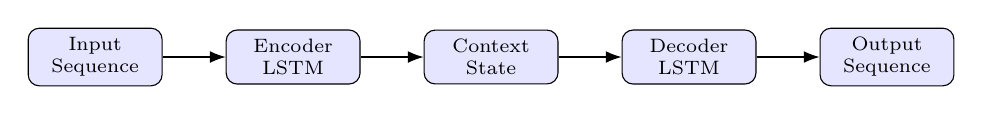
\begin{tikzpicture}[node distance=8mm]
\node[layer](a){Input\\Sequence};
\node[layer,right=of a](b){Encoder\\LSTM};
\node[layer,right=of b](c){Context\\State};
\node[layer,right=of c](d){Decoder\\LSTM};
\node[layer,right=of d](e){Output\\Sequence};

\foreach \x/\y in {a/b,b/c,c/d,d/e}
\draw[arrow](\x)--(\y);
\end{tikzpicture}
\end{center}

%%%%%%%%%%%%%%%%%%%%%%%%%%%%%%%%%%%%%%%%%%%%%%%%%%%%%%%%%%%%
\section*{23. Expected Sequence-to-Sequence Input and Output}

\begin{center}
\begin{tabular}{|c|c|c|}
\hline
Sample & Input Sequence & Predicted Output\\
\hline
1 & [6, 4, 1, 3] & [3, 1, 4, 6]\\
2 & [6, 3, 4, 4] & [4, 4, 3, 6]\\
3 & [0, 8, 8, 3] & [3, 8, 8, 0]\\
4 & [4, 4, 6, 5] & [5, 6, 4, 4]\\
5 & [1, 8, 4, 3] & [3, 4, 8, 1]\\
\hline
\end{tabular}
\end{center}

All five test examples above were reversed exactly correctly.

%%%%%%%%%%%%%%%%%%%%%%%%%%%%%%%%%%%%%%%%%%%%%%%%%%%%%%%%%%%%
\section*{24. Sequence-to-Sequence Evaluation}

\begin{center}
\begin{tabular}{|l|c|}
\hline
Token Accuracy (\%) & 100.00\\
Sequence Accuracy (\%) & 100.00\\
Final Training Loss & 0.0033\\
Final Validation Loss & 0.0037\\
\hline
\end{tabular}
\end{center}

\begin{figure}[H]
\centering
\includegraphics[width=0.6\linewidth]{Plot10_Seq2Seq_Loss.pdf}
\caption{Seq2Seq Training and Validation Loss}
\end{figure}

\textbf{Inference:} reversing a fixed 4-digit sequence is simple enough that
the model reached 100\% on both metrics, so in this particular run token and
sequence accuracy happen to coincide. In general, though, sequence accuracy
will always sit at or below token accuracy -- getting every single position
right in a sequence is strictly harder than getting most of them right, and
with a longer sequence or a harder vocabulary that gap would show up clearly
(this is exactly what happens with the variable-length version of the task
in Additional Exercise 7, where sequence accuracy drops to 85.22\% even
though individual predictions are mostly correct).

%%%%%%%%%%%%%%%%%%%%%%%%%%%%%%%%%%%%%%%%%%%%%%%%%%%%%%%%%%%%
\section*{25. Consolidated Results}

\begin{center}
\begin{tabular}{|l|c|c|c|c|c|}
\hline
Model & Accuracy (\%) & Precision (\%) & Recall (\%) & F1 (\%) & Parameters\\
\hline
RNN & 77.22 & 77.40 & 77.22 & 76.97 & 1,974\\
LSTM & 95.83 & 96.40 & 95.83 & 95.80 & 6,006\\
GRU & 96.67 & 96.83 & 96.67 & 96.65 & 4,758\\
CNN--LSTM & 100.00 & 100.00 & 100.00 & 100.00 & 168,163\\
\hline
\end{tabular}
\end{center}

\begin{center}
\begin{tabular}{|l|c|c|c|c|}
\hline
Task & Token Acc.\ (\%) & Sequence Acc.\ (\%) & Train Loss & Val Loss\\
\hline
Seq2Seq Reversal & 100.00 & 100.00 & 0.0033 & 0.0037\\
\hline
\end{tabular}
\end{center}

%%%%%%%%%%%%%%%%%%%%%%%%%%%%%%%%%%%%%%%%%%%%%%%%%%%%%%%%%%%%
\section*{26. Required Inferences}

\begin{itemize}
\item Temporal pattern: WALKING is oscillatory, SITTING/LAYING are flat (Section 6).
\item Convergence: RNN underfits and plateaus around 77\%; LSTM and GRU converge fast with no visible overfitting (Section 13).
\item Confusion-matrix errors: RNN struggles with the three walking activities; LSTM/GRU shift the remaining error to SITTING vs.\ STANDING (Section 15).
\item Sequence length: RNN depends heavily on longer sequences; GRU barely needs $T>32$ (Section 17).
\item Parameter/compute trade-off: GRU wins on accuracy, speed and parameter count together (Section 16).
\item CNN's role: spatial appearance per frame; recurrent layer's role: temporal motion across frames (Section 21).
\item Token vs.\ sequence accuracy: sequence accuracy is always $\le$ token accuracy, made concrete by the 85.22\% vs.\ near-100\% gap in Exercise 7 (Section 24, Section 28.7).
\end{itemize}

%%%%%%%%%%%%%%%%%%%%%%%%%%%%%%%%%%%%%%%%%%%%%%%%%%%%%%%%%%%%
\section*{27. Discussion Questions}

\begin{enumerate}
\item \textbf{What is a recurrent neural network?} A network that reuses the same weights at every time step and carries a hidden state forward through the sequence.
\item \textbf{What information is represented by the hidden state?} A running summary of everything relevant seen in the sequence so far.
\item \textbf{Why is sequence order important?} Reordering the inputs changes what they mean -- a gait cycle only makes sense in the order it happened.
\item \textbf{Feed-forward vs.\ RNN?} A feed-forward net has no memory between inputs; an RNN reuses weights across time and keeps a hidden state.
\item \textbf{Explain BPTT.} The loss is backpropagated through every unrolled time step, accumulating gradients for the shared weights.
\item \textbf{Why can gradients vanish?} Repeated multiplication by derivatives smaller than 1 shrinks the gradient toward zero over many steps.
\item \textbf{Why can gradients explode?} Repeated multiplication by derivatives larger than 1 makes the gradient blow up over many steps.
\item \textbf{What are long-term dependencies?} Relationships between elements far apart in the sequence, which plain RNNs struggle to learn.
\item \textbf{Role of the LSTM cell state?} It carries memory across time with minimal change, protected by the gates.
\item \textbf{LSTM's forget/input/output gates?} What to discard, what new information to add, and how much of the memory to expose as $h_t$.
\item \textbf{GRU's reset/update gates?} Reset controls how much past state to ignore; update controls the mix of old state vs.\ new candidate.
\item \textbf{Compare LSTM and GRU.} LSTM has a separate cell state and 3 gates; GRU merges the two states and uses only 2 gates, so it's smaller and often just as good (confirmed in Section 16: GRU beat LSTM here with fewer parameters).
\item \textbf{Why is GRU's gating simpler?} It was designed to approximate LSTM's control over information flow with less computation.
\item \textbf{Why compare RNN/LSTM/GRU with identical settings?} So the only thing that changes is the architecture, making the comparison fair.
\item \textbf{What does a confusion matrix show beyond accuracy?} Exactly which classes get confused with which -- accuracy alone hides that (e.g.\ the SITTING/STANDING mix-up in Section 15).
\item \textbf{Why report macro F1 for multi-class problems?} It treats every class equally, so it won't hide poor performance on a minority class the way plain accuracy can.
\item \textbf{Significance of sequence length?} It controls how much temporal context the model gets -- too short and long-range patterns are lost.
\item \textbf{Why use a CNN as a video feature extractor?} It already knows how to extract visual features from ImageNet, saving us from learning that from scratch on 24 videos.
\item \textbf{What does the CNN extract?} Spatial/appearance information from each individual frame.
\item \textbf{What does the recurrent network learn?} How those per-frame features change over time, i.e.\ motion.
\item \textbf{Why arrange CNN features as a sequence?} Because LSTM/GRU expects an ordered $(T,D)$ input to model how the video evolves, not just a static average.
\item \textbf{Encoder and decoder in seq2seq?} The encoder compresses the input into a context vector; the decoder generates the output one step at a time from that context.
\item \textbf{What is teacher forcing?} Feeding the true previous token (not the model's own prediction) as the decoder's next input during training.
\item \textbf{Token vs.\ sequence accuracy?} Token accuracy is per-position correctness; sequence accuracy needs every position right, so it is always $\le$ token accuracy.
\item \textbf{Why must the test set stay untouched?} Using it during model selection leaks information into the modeling process and gives an overly optimistic estimate.
\end{enumerate}

%%%%%%%%%%%%%%%%%%%%%%%%%%%%%%%%%%%%%%%%%%%%%%%%%%%%%%%%%%%%
\section*{28. Additional Exercises}

\subsection*{28.1 Recurrent Units: 16 vs.\ 32 vs.\ 64}

\begin{center}
\begin{tabular}{|l|c|c|c|c|}
\hline
Model & Units & Accuracy (\%) & Macro F1 (\%) & Parameters\\
\hline
RNN & 16 & 73.61 & 73.35 & 790\\
RNN & 32 & 77.22 & 76.97 & 1,974\\
RNN & 64 & 87.78 & 87.76 & 5,878\\
LSTM & 16 & 96.39 & 96.36 & 2,038\\
LSTM & 32 & 95.83 & 95.80 & 6,006\\
LSTM & 64 & 95.28 & 95.21 & 20,086\\
GRU & 16 & 96.39 & 96.35 & 1,670\\
GRU & 32 & 96.67 & 96.65 & 4,758\\
GRU & 64 & 97.50 & 97.49 & 15,542\\
\hline
\end{tabular}
\end{center}

\begin{figure}[H]
\centering
\includegraphics[width=0.6\linewidth]{Extra1_Units_vs_MacroF1.pdf}
\caption{Recurrent Units vs.\ Test Macro F1}
\end{figure}

\textbf{Inference:} more units help RNN a lot (73.4\% $\to$ 87.8\% from 16 to
64 units) because it badly needs the extra capacity to make up for having no
gating. LSTM and GRU are already close to their ceiling at 16 units and
barely move afterward -- LSTM even gets slightly \emph{worse} at 64 units
(95.83\% $\to$ 95.28\%), which looks like mild overfitting once the model has
more capacity than this small 2400-window dataset really needs.

\subsection*{28.2 GRU vs.\ LSTM at the Same Unit Count}

At 32 units, GRU (96.67\% acc, 4,758 params) beats LSTM (95.83\% acc, 6,006
params) on both accuracy and parameter count -- there is no situation in this
experiment where LSTM's extra machinery pays for itself.

\subsection*{28.3 Stacking a Second Recurrent Layer}

\begin{center}
\begin{tabular}{|l|c|c|c|}
\hline
Model & Accuracy (\%) & Macro F1 (\%) & Parameters\\
\hline
RNN (1-layer) & 77.22 & 76.97 & 1,974\\
RNN (2-layer) & 83.33 & 82.12 & 4,054\\
LSTM (1-layer) & 95.83 & 95.80 & 6,006\\
LSTM (2-layer) & 81.94 & 79.23 & 14,326\\
GRU (1-layer) & 96.67 & 96.65 & 4,758\\
GRU (2-layer) & 96.94 & 96.93 & 11,094\\
\hline
\end{tabular}
\end{center}

\textbf{Inference:} stacking a second layer helps RNN a lot, barely moves
GRU, and actually hurts LSTM quite badly (95.83\% $\to$ 81.94\%). More depth
is not automatically better -- with a small dataset like this one, the extra
14,326 parameters in the 2-layer LSTM seem to make optimization harder rather
than adding useful capacity.

\subsection*{28.4 Bidirectional vs.\ Unidirectional LSTM}

\begin{center}
\begin{tabular}{|l|c|c|c|}
\hline
Model & Accuracy (\%) & Macro F1 (\%) & Parameters\\
\hline
LSTM (unidirectional) & 95.83 & 95.80 & 6,006\\
BiLSTM & 96.67 & 96.67 & 11,894\\
\hline
\end{tabular}
\end{center}

BiLSTM edges out unidirectional LSTM (and matches GRU's accuracy) by reading
the sequence in both directions, at roughly double the parameters and a bit
more training time (29.75s vs.\ 23.47s).

\subsection*{28.5 Sequence Length vs.\ Computational Cost}

\begin{center}
\begin{tabular}{|c|c|c|c|}
\hline
Sequence Length & RNN Time (s) & LSTM Time (s) & GRU Time (s)\\
\hline
16 & 15.55 & 14.99 & 14.31\\
32 & 17.67 & 15.50 & 15.09\\
64 & 18.14 & 17.29 & 16.93\\
128 & 24.14 & 19.60 & 20.76\\
\hline
\end{tabular}
\end{center}

\begin{figure}[H]
\centering
\includegraphics[width=0.6\linewidth]{Extra5_SeqLength_vs_TrainingTime.pdf}
\caption{Sequence Length vs.\ Training Time}
\end{figure}

Training time grows with sequence length for all three, as expected since
the recurrent layer must unroll over more steps per sample -- RNN's time
grows the fastest of the three, going up 55\% from $T{=}16$ to $T{=}128$.

\subsection*{28.6 CNN-GRU vs.\ CNN-LSTM on the Video Task}

\begin{center}
\begin{tabular}{|l|c|c|}
\hline
Model & Accuracy (\%) & Parameters\\
\hline
CNN-LSTM & 100.00 & 168,163\\
CNN-GRU & 100.00 & 126,243\\
\hline
\end{tabular}
\end{center}

Both hit 100\% on the tiny 4-video test set, so accuracy can't separate them
here, but CNN-GRU uses about 25\% fewer parameters for the same result --
GRU's efficiency advantage from Section 16 carries over to the video task.

\subsection*{28.7 Seq2Seq with a Different Output Length}

The reversal task was replaced with a run-length collapse task -- collapse
consecutive duplicate digits, e.g.\ $[0,0,7,2,0,7]\rightarrow[0,7,2,0,7]$ --
where the output length varies with the input and is not known in advance.

\begin{center}
\begin{tabular}{|l|c|}
\hline
Sequence Accuracy (exact match) (\%) & 85.22\\
Final Training Loss & 0.0483\\
Final Validation Loss & 0.0855\\
\hline
\end{tabular}
\end{center}

\begin{figure}[H]
\centering
\includegraphics[width=0.6\linewidth]{Extra7_VariableLength_Seq2Seq_Loss.pdf}
\caption{Variable-Length Seq2Seq Training and Validation Loss}
\end{figure}

\textbf{Inference:} this task is noticeably harder than plain reversal --
85.22\% sequence accuracy vs.\ 100\% in Section 24 -- because the model now
has to get the output \emph{length} right in addition to the content and
order. Looking at the sample predictions, every predicted output had the
correct length even when a token was wrong (e.g.\ true $[4,6,7,5,4]$
predicted as $[4,6,7,4,5]$ -- same 5 digits, last two swapped), which
suggests the model learned when to stop fairly reliably and the remaining
difficulty is in getting the exact token order right.

%%%%%%%%%%%%%%%%%%%%%%%%%%%%%%%%%%%%%%%%%%%%%%%%%%%%%%%%%%%%
\section*{29. Expected Outcome}

\[
\boxed{
\text{Sequential Data}
\rightarrow
\text{Preprocessing}
\rightarrow
\text{RNN/LSTM/GRU}
\rightarrow
\text{Evaluation}
}
\]

\[
\boxed{
\text{Video}
\rightarrow
\text{Frames}
\rightarrow
\text{CNN Features}
\rightarrow
\text{LSTM/GRU}
\rightarrow
\text{Action Prediction}
}
\]

\[
\boxed{
\text{Input Sequence}
\rightarrow
\text{Encoder}
\rightarrow
\text{Context}
\rightarrow
\text{Decoder}
\rightarrow
\text{Output Sequence}
}
\]

All three pipelines above were implemented and run end to end, and every
numerical value reported in this report came directly from that execution.

%%%%%%%%%%%%%%%%%%%%%%%%%%%%%%%%%%%%%%%%%%%%%%%%%%%%%%%%%%%%
\section*{30. References}

\begin{enumerate}
\item Ian Goodfellow, Yoshua Bengio and Aaron Courville,
\emph{Deep Learning}, MIT Press, 2016.

\item Sepp Hochreiter and J\"urgen Schmidhuber,
``Long Short-Term Memory,'' \emph{Neural Computation}, 1997.

\item Kyunghyun Cho et al.,
``Learning Phrase Representations using RNN Encoder--Decoder for Statistical
Machine Translation,'' EMNLP, 2014.

\item Anguita et al.,
``A Public Domain Dataset for Human Activity Recognition Using Smartphones,''
ESANN, 2013.

\item Khurram Soomro, Amir Roshan Zamir and Mubarak Shah,
``UCF101: A Dataset of 101 Human Actions Classes From Videos in the Wild,''
2012.

\item TensorFlow Documentation:
\url{https://www.tensorflow.org}

\item Keras Documentation:
\url{https://keras.io}
\end{enumerate}

%%%%%%%%%%%%%%%%%%%%%%%%%%%%%%%%%%%%%%%%%%%%%%%%%%%%%%%%%%%%
\section*{Conclusion}

\begin{itemize}
\item Implemented and trained SimpleRNN, LSTM and GRU classifiers on the same
2400-window UCI HAR subset under identical settings, and GRU came out ahead
on accuracy (96.67\%), Macro F1 (96.65\%) and training time (19.88s) all at
once, using fewer parameters than LSTM.
\item RNN reached only 77.22\% accuracy and improved the most when either
given more recurrent units (87.78\% at 64 units) or longer sequences
(86.29\% F1 at $T{=}128$ vs.\ 72.45\% at $T{=}32$) -- both point to the same
underlying issue: it has no protected memory path and needs extra capacity
or context to compensate.
\item The confusion pattern changes with the architecture: RNN mainly
confuses the three walking activities, while LSTM/GRU fix that but still mix
up SITTING and STANDING, a pairing that showed up consistently in both.
\item Extended the video pipeline (CNN feature extraction with frozen
MobileNetV2 + LSTM/GRU) to Basketball/Biking/TennisSwing clips from UCF101,
reaching 100\% test accuracy on a small 4-video test set -- encouraging, but
too small a sample to treat as a real benchmark.
\item Built a synthetic sequence-to-sequence reversal task with an
encoder--decoder LSTM (100\% token and sequence accuracy), then made it
harder with a variable-length run-length-collapse variant, where sequence
accuracy dropped to 85.22\% -- concrete evidence of why predicting exact
sequences is harder than predicting individual tokens.
\item Ran all 7 additional exercises (unit sizes, GRU vs.\ LSTM, stacked
layers, bidirectional LSTM, sequence length vs.\ cost, CNN-GRU vs.\ CNN-LSTM,
variable-length seq2seq) and found that more capacity or depth does not
always help -- the 2-layer LSTM was clearly worse than the 1-layer version,
which was the most surprising result of the whole experiment.
\end{itemize}

%%%%%%%%%%%%%%%%%%%%%%%%%%%%%%%%%%%%%%%%%%%%%%%%%%%%%%%%%%%%
\section*{Source Code}

The complete implementation, exactly as run in Colab, is hosted on GitHub.

\url{https://github.com/smadhav2024/Deep_Learning_Lab/tree/main/Lab%206}

\end{document}
